实际数组传递同样是复现契约的一部分。第二轮启动时，Windows重新生成的六份候选输入中，噪声与导数探测数组相同，但对数均匀数组有82/49152个元素不同，最大差约$4.44\times10^{-16}$，因此原协议拒绝启动机制工作流。随后传递原始封存文件，按原哈希和容差完成了下述测量；原启动失败与候选数组仍保留。相同种子和依赖版本不能替代实际数组校验，核验本身也未确定底层数学库差异的因果来源。

\subsection{Windows有限机制测量}
独立机制协议在G1、G2、L1上各使用@@TAPES@@份主随机输入，比较窗口4/16、链数分配及预先规定的G2 RWM步长对照。CPU与CUDA各完成96个工作流；每个工作流包括首次审计、@@REPLAYS@@次交错缓存重放和探针后重放。全部960份保存路径通过独立NumPy参考核验，接受事件零失配，最大绝对路径差为$@@PATH_ERROR@@$。技术重放、窗口变体和跨设备副本均不增加独立输入数。

测量使用同一台Windows 11计算机的Ryzen 7 9800X3D和RTX 5080，torch主机线程设为4，CUDA使用float64并显式同步。桌面显示负载仍存在，不将线程数等同独占物理核心数。表\ref{tab:windows-mechanism}给出全部配置的描述性比值；它们来自三次缓存sample时间中位数之比，既不是完整推断成本比，也不是跨独立重复的置信区间。

\begin{table}[htbp]\centering\small
\begin{tabular}{lrrl}\toprule
设备/执行器 & 配对数 & 比值大于1 & 全部比值范围\\\midrule
@@TABLE@@
\bottomrule\end{tabular}
\caption{机制协议的同核缓存执行比值：同组顺序时间除以时间执行器时间。全部120个时间执行配置均保留；quasi-DEER对应MALA，Picard对应RWM。每模型仅两份独立输入，配对数不能解释为独立实验数。}
\label{tab:windows-mechanism}
\end{table}

quasi-DEER每个输出转移对应@@FORWARD_MALA@@次前向映射及@@JVP_MALA@@次JVP；Picard为@@FORWARD_RWM@@次前向映射（图\ref{fig:windows-mechanism}）。这些计数包括拒绝自环，均高于顺序执行的一次前向映射；映射与JVP不是等价浮点工作量，不能简单相加。每端6个工作流完全零接受，全部保留。例如G2/RWM步长1.0的第一份输入，在窗口4/16下可一次确认整个窗口，同时没有接受移动。因此较长的确认前缀可以由自环产生，并不表示更有效的后验探索。

\begin{figure}[htbp]\centering
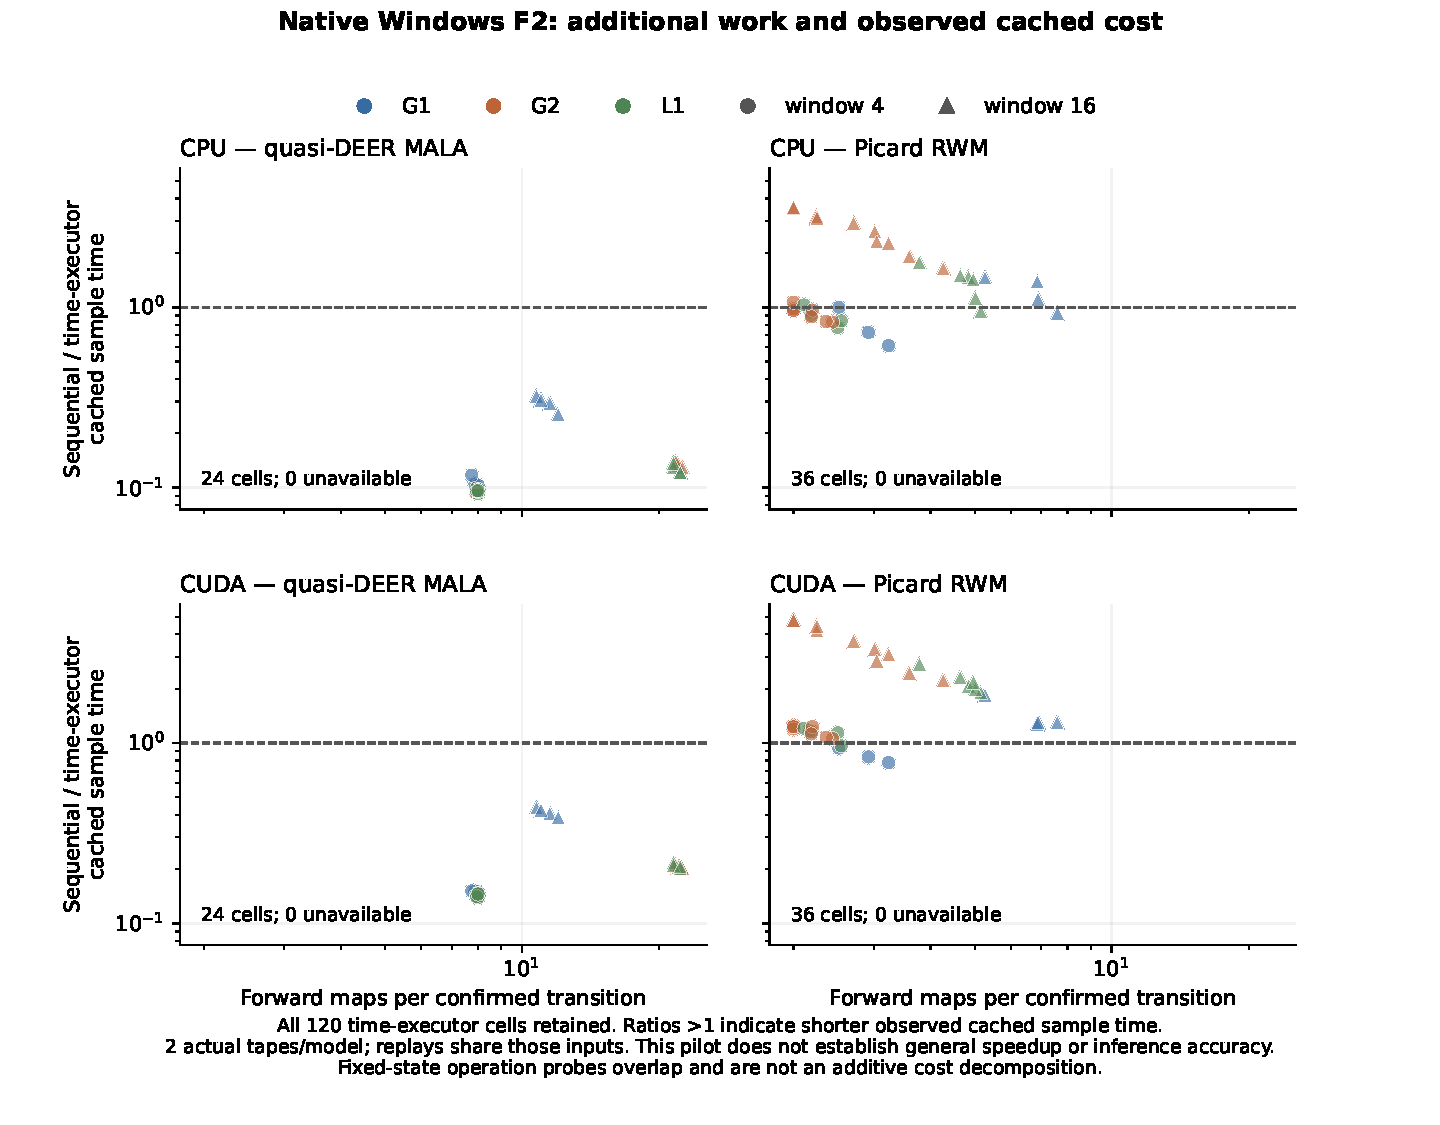
\includegraphics[width=\linewidth]{../../figures/windows-mechanism-pilot-v1/work-and-cached-cost.pdf}
\caption{Windows机制测量中的重复求值与缓存成本。每点为一个配置与实际输入的组合，共120点，部分重叠；颜色区分目标，点形区分窗口。上下行为CPU/CUDA，左右列为quasi-DEER/Picard。纵轴大于1表示指定缓存执行较短；横轴包括拒绝自环。三次技术重放不扩充独立样本量，图中没有推断精度或统计区间。操作探针存在重叠，不用于构造可加的独占耗时分解。}
\label{fig:windows-mechanism}
\end{figure}

预先规定的等512个总输出对照提供了另一种解释边界。在G2、L1的两份输入及两个设备上，16条各32步的顺序链均比单条512步、窗口16的Picard链更快，后者时间为前者的@@ALLOCATION_MIN@@--@@ALLOCATION_MAX@@倍。这8个技术对照说明链数分配会改变执行吞吐；两种分配的轨迹长度、初始化份数及探索能力不同，不能解释为相同推断精度下的优劣。图示的额外工作量与quasi-DEER减速相容，但不足以唯一归因于JVP、扫描或主机控制；固定状态操作探针与生产路径不同，同步及嵌套操作也使各阶段不能相加还原总时间。

\subsection{批次运行与安装的实测范围}
另一个Windows技术批次完成@@MAIN_TASKS@@项主任务和@@CACHE_TASKS@@项缓存探测（@@CACHE_CALLS@@次调用），包含最大形状、进程集合管理和终态恢复检查。接收端对保存MH数组独立重放，并核对函数与R诊断；这没有新增正式推断重复。@@DIAG_ROWS@@条函数诊断中仍有@@BAD_RHAT@@条$\hat R>1.01$及@@TAIL_NULL@@条tail ESS不可判定，不能将运行成功解释为收敛。该批次支持其封存运行器的技术能力；后续正式协议适配器的独立Windows验收与充分预算比较仍需完成。

Python 0.2.0.dev2与R 0.2.0.9002候选已在Windows新建依赖环境和仓库外完成安装核验，覆盖CPU/CUDA MH和R批量入口。默认R包检查与显式集成测试分别保存；成功检查不隐去此前安装和locale失败。接收端核对源码、sdist、wheel与R包中17个模块，并从保存RDS重建诊断，没有在Mac重新测量CUDA。该证据不涵盖原生Windows的JAX/Stan安装、GPU NUTS或第三方团队的独立复现。
